\documentclass[serif, aspectratio=169]{beamer}
%\documentclass[serif]{beamer}  % for 4:3 ratio

%\RequirePackage{minted2}
\usepackage[T1]{fontenc} 
\usepackage[utf8]{inputenc}
\usepackage{fourier} % see "http://faq.ktug.org/wiki/uploads/MathFonts.pdf" for other options
\usepackage{hyperref}
\usepackage{latexsym,amsmath,xcolor,multicol,booktabs,calligra}
\usepackage{graphicx,pstricks,listings,stackengine}
\usepackage{lipsum}
\usepackage{../../../TEMPLATES/template_style}

%imports customs%
\usepackage{caption}    % for subfigures
\usepackage{subcaption} % for subfigures
\usepackage{ragged2e}
\usepackage{booktabs,makecell}
\usepackage{colortbl}
\usepackage{multirow}
\usepackage{cite}
\usepackage{tcolorbox}
\usepackage[sort,authoryear]{natbib}

\author{Julien Bezançon}

\title{Phraseology}
\subtitle{CM 1~: Welcome and Introduction}

\institute{julien.bezancon@univ-lorraine.fr / \url{https://julienbez.github.io}}

\date{}

% defs
\def\cmd#1{\texttt{\color{red}\footnotesize $\backslash$#1}}
\def\env#1{\texttt{\color{blue}\footnotesize #1}}

% set colors
\definecolor{hkustyellow}{RGB}{167, 131, 55}
\definecolor{hkustblue}{RGB}{0, 56, 116}
\definecolor{hkustred}{RGB}{209, 51, 59}

\lstset{
    basicstyle=\ttfamily\small,
    keywordstyle=\bfseries\color{deepblue},
    emphstyle=\ttfamily\color{deepred},    % Custom highlighting style
    stringstyle=\color{deepgreen},
    numbers=left,
    numberstyle=\small\color{halfgray},
    rulesepcolor=\color{red!20!green!20!blue!20},
    frame=shadowbox,
}

\begin{document} %  --- --- --- --- --- --- --- --- --- --- --- --- 

\begin{frame}[noframenumbering,plain]
    \titlepage
    \vspace*{-0.6cm}
    \begin{figure}[htpb]
        \begin{center}
            \hspace{0.3cm}
            
\includegraphics[width=0.7\columnwidth]{../../../IMAGES/loria_idmc.png}
        \end{center}
    \end{figure}
\end{frame}

% \begin{frame}    
%     \tableofcontents[sectionstyle=show,
%     subsectionstyle=show/shaded/hide,
%     subsubsectionstyle=show/shaded/hide]
% \end{frame}

\section{Before we start...}

\begin{frame}{About me} %Julien Bezançon
    \begin{minipage}{0.45\columnwidth}
        \begin{figure}
            
\includegraphics[width=0.7\columnwidth]{../../../FIGURES/photos/profile_thug.jpeg}
        \end{figure}
    \end{minipage}
    \begin{minipage}{0.45\columnwidth}
        \begin{block}{You will see me in...}
            \vspace{5pt}
            \begin{itemize}
                \item Prompt Engineering \hfill M2
                \item Software Projects \hfill M2
                \item Written Corpora \hfill M2
            \end{itemize}
        \end{block}
    \end{minipage}
\end{frame}

\begin{frame}{About this course} %-- 8 weeks, 4 hours a week
    \begin{block}{7 lectures}
        \begin{itemize}
            \item Phraseology and Multiword expressions
            \item Fixation, Defixation and Refixation
            \item Multiword expressions and NLP
        \end{itemize}
    \end{block}
    \pause
    \vfill
    \begin{block}{Evaluation mode}
        \begin{itemize}
            \item Oral session (50~\%) 
            \item Final exam (50~\%)
        \end{itemize}
    \end{block}
    \pause
    \vfill
    \hfill \textbf{Final exam on last lecture}
\end{frame}

\begin{frame}{References for this course}
    \begin{block}{}

    \end{block}
\end{frame}

\section{Introduction}

\begin{frame}{What is Phraseology ?}
    \begin{block}{Wikipedia Definition\footnote{\url{https://en.wikipedia.org/wiki/Phraseology}}}
        \begin{tcolorbox}
            Phraseology is the study of set or fixed expressions, such as idioms, phrasal verbs, and other types of multi-word lexical units (often collectively referred to as phrasemes), in which the component parts of the expression take on a meaning more specific than, or otherwise not predictable from, the sum of their meanings when used independently.
        \end{tcolorbox}
    \end{block}
    \vfill
    \begin{center}
        \Large
        Phraseology studies fixed sequences of words. \\
        Several words, but only one meaning.
    \end{center}s
\end{frame}

\begin{frame}{A bit of History}
    \begin{block}{Phraseology is a young discipline}
        \begin{itemize}
            \item First appearances: end of 19\textsuperscript{th} - begining of 20\textsuperscript{th} century
            \item Term coined by Charles Bally in 1909
            \item since 1970~: "phraseological boom" \citep{} %granger and meunier, 2008
        \end{itemize}
    \end{block}
    \vfill
    \begin{block}{Phraseology is at a crossroad between several disciplines}
        \begin{itemize}
            \item Phraseology \textbf{is not} just a subdomain of syntax
            \item Phraseology \textbf{is not} just a subdomain of lexicology
            \item Phraseology \textbf{is} a central domain of language sciences \citep{} %agnes tutin https://shs.cairn.info/revue-langages-2025-3-page-7?lang=fr
        \end{itemize}
    \end{block}
\end{frame}

\begin{frame}{Terminological Nightmare}
    \begin{block}{}
    \textit{clause, conventional collocation, colligation, discourse structuring device, formulae idiom, irreversible binomial, phrase, prefab, quotation, simile, ...}
    \end{block}
    \vfill
    \begin{block}{Consequences}
        \begin{itemize}
            \item Lots of confusions / repetitions
            \item Incompatible properties \citep{} %gross 1996
        \end{itemize}
    \end{block}
    \vfill
    \begin{center}
        \Large
        For any given classification, there will always be \\ objects that fall outside of it \citep{}. % Heinz 1993
    \end{center}
\end{frame}

\begin{frame}{Conventional names}
    \begin{block}{}
        \begin{itemize}
            \item Idiom
            \item Phraseme
            \item Set phrase
            \item Fixed expression
            \item Multiword expression
        \end{itemize}
    \end{block}
    \vfill
    \begin{center}
        \Large
        During this class, we will mainly use the term \\ "Multiword expression" (MWE).
    \end{center}
\end{frame}

\section{Multiword Expressions}

\begin{frame}{How to define a MWE ?}
    \begin{block}{\citep{} definition} %Bally, 1909
        "phrases that function as units rather than as series"\footnote{"locutions qui ont le caractère d'unités plutôt que de séries"}
    \end{block}
    \vfill
    \begin{block}{\citep{} key parameters of a MWE}
        \begin{itemize}
            \item the nature of its components (either lexical entries and grammatical paterns)
            \item the number of components in it
            \item its frequency and its status (is it conventionalized ?)
            \item the distance between its components
            \item the lexical and syntactic flexibility of its components
            \item the semantic role of its components and its level of compositionnality
        \end{itemize}
    \end{block}
\end{frame}

\begin{exoframe}{Exercise Time !}
    \begin{block}{Study the MWEs within the following sentences}
        \begin{itemize} \color{white}
            \item Max kicked the bucket
            \item Max and Marie kicked the bucket
            \item I will look these student numbers up
            \item I love them all, kith and kin alike
            \item My bad for adding fuel on the fire
        \end{itemize}
    \end{block}
    \pause
    \vfill
    \begin{center}
        \Large
        Can you identify some properties shared by all these MWEs ?
    \end{center}
\end{exoframe}

\begin{frame}{MWE properties}
    \begin{block}{No clear consensus, but some shared properties}
        \begin{itemize}
            \item[1.] A MWE has several components
            \item[2.] A MWE is somewhat fixed
            \item[3.] A MWE has a somewhat idiomatic meaning
        \end{itemize}
    \end{block}
    \vfill
    \begin{center}
        \Large
        Parameters: the things we use to study a MWE. \\
        Properties: the rules supposedly shared among all MWEs.
    \end{center}
\end{frame}

\begin{frame}{1. A MWE has several components}
    \begin{block}{A MWE contains several units}
        \begin{itemize}
            \item In latin languages, 1 unit $\approx$ 1 word
            \item Word: a sequence of characters delimited by spaces
        \end{itemize}
    \end{block}
    \vfill
    \begin{block}{Limits}
        \begin{itemize}
            \item \textit{Hot Dog} (english): two words ?
            \item \textit{Evlerimdekiler}\footnote{those who are in the houses} (turkish): one word ?
            \item \textit{faire d'une pierre deux coups}\footnote{killing two birds with one stone} (french): several words ?
        \end{itemize}
    \end{block}
\end{frame}

\begin{frame}{1. A MWE has several components}
    \begin{block}{}
        \wordbox{Max} \wordbox{kicked} \wordbox{the} \wordbox{bucket} \\
        \wordbox{Max} \wordbox{kicked the bucket} \\ 
        \wordbox{Max} \wordbox{and} \wordbox{Marie} \wordbox{kicked the bucket} \\
    \end{block}
    \vfill
    \begin{block}{}
        \wordbox{My} \wordbox{bad} \wordbox{for} \wordbox{adding} \wordbox{fuel} \wordbox{on} \wordbox{the} \wordbox{fire} \\
        \wordbox{My} \wordbox{bad} \wordbox{for} \wordbox{adding fuel on the fire} \\ 
    \end{block}
\end{frame}

\begin{frame}{2. A MWE is somewhat fixed}
    \begin{block}{The components of a MWE are stables}
        \begin{itemize}
            \item \textit{Fish and Chips}
            \item \textit{May the force be with you}
            \item \textit{I will kill / killed two birds with one stone}
        \end{itemize}
    \end{block}
    \vfill
    \begin{block}{Limits}
       \begin{itemize}
        \item Some MWEs can accept slight variations
        \item Some MWEs can accept word substitutions
       \end{itemize} 
    \end{block}
\end{frame}

\begin{frame}{2. A MWE is somewhat fixed}
    \begin{table}
        \centering
        \renewcommand{\arraystretch}{1.5} 
        \begin{tabular}{|l|l|c|}
            \hline
            \textbf{Variation} & \textbf{MWE} & \textbf{valid ?} \\
            \hline
            Base         & Max kicked the bucket & yes \\
            \hline
            Tense        & Max is going to kick the bucket & yes \\
            \hline
            Adverb       & Max will kick the bucket in a few hours & yes \\
            \hline
            Insertion    & Max has unfortunatly kicked the bucket & yes \\
            \hline
            Passivation  & The bucket of Max was kicked & no \\
            \hline
            Clivage      & This is the bucket that Max kicked & no \\
            \hline
            Substitution & Max kicked the vessel / pot & no \\
            \hline
        \end{tabular}
        \caption*{Adapted from \citep{}}
    \end{table}
\end{frame}

% \begin{frame}{2. A MWE is somewhat fixed}
%     \begin{block}{Multiple forms, same meaning}
%         \begin{itemize}
%             \item \textit{Ce n'ai pas le pingouin qui glisse le plus loin}
%             \item \textit{Ce n'ai pas le couteau le plus aiguisé du tirroir}
%             \item \textit{Ce n'ai pas le fromage le plus affiné du terroir}
%             \vspace{10pt}
%             \item \textit{Il y a anguille sous roche}
%             \item \textit{Il y a baleine sous gravier}
%         \end{itemize}
%     \end{block}
% \end{frame}

\begin{frame}{3. A MWE has a somewhat idiomatic meaning}
    \begin{block}{MWEs tend to be non-compositional}
        \begin{itemize}
            \item Several units, one meaning
            \item MWE Meaning $\ne$ sum of its components
        \end{itemize}
    \end{block}
    \vfill
    \begin{block}{Limits}
        \begin{itemize}
            \item Semi-compositional MWEs (\textit{adding fuel on the fire})
            \item Fully-compositional MWEs (\textit{to make a decision})
        \end{itemize}
    \end{block}
\end{frame}

\begin{frame}{3. A MWE has a somewhat idiomatic meaning}
    \begin{block}{Semantic opacity of a MWE}
        \begin{itemize}
            \item You can not guess a MWE meaning from its components
            \begin{itemize}
                \item your MWE is non-compositional
            \end{itemize}
            \vspace{10pt}
            \item You can partially guess a MWE meaning from some of its components
            \begin{itemize}
                \item your MWE is semi-compositional
            \end{itemize}
            \vspace{10pt}
            \item You can guess a MWE meaning from its components
            \begin{itemize}
                \item yout MWE is fully-compositional
            \end{itemize}
        \end{itemize}
    \end{block}
    \begin{center}
        \Large
        Reality: it's a \textit{continuum}.
    \end{center}
\end{frame}

\begin{exoframe}{}
    \begin{center}
        \Large
        One last property: the most important one. \\
        \vspace{10pt}
        Take your guesses !
    \end{center}
\end{exoframe}

\begin{frame}{4. A MWE is Conventionalized}
    \begin{block}{Conventionality}
        \begin{itemize}
            \item Conventionalized MWE: known by a group of individuals
            \item \textbf{Conventionality is a trait shared by all MWEs}
        \end{itemize}
    \end{block}
    \vfill
    \begin{block}{About the notion of "group of individuals"}
        \begin{itemize}
            \item The population of a region, a state, a country, etc
            \item The individuals inside this class
        \end{itemize}
    \end{block}
\end{frame}

\section{Multiword Expressions and NLP}

\begin{exoframe}{}
    \begin{center}
        \Large
        Let's start with a question. \\
        \vspace{10pt}
        Do you think it is useful to process MWEs in NLP ?
    \end{center}
\end{exoframe}

\begin{frame}{MWEs in NLP}
    \begin{block}{Interests}
        \begin{itemize}
            \item Better contextualization 
            \begin{itemize}
                \item \citep{}: XX~\% of MWEs in english texts
                \item Can resolve many ambiguities
            \end{itemize}
            \vspace{10pt}
            \item Human writing VS machine writing
            \begin{itemize}
                \item Does LLMs use fewer MWEs than humans ?
            \end{itemize}
            \vspace{10pt}
            \item (Much) better translations
            \begin{itemize}
                \item hang on ! $\Rightarrow$ pends-toi
                \item it's raining cats and dogs $\Rightarrow$ il pleut des chats et des chiens
            \end{itemize}
        \end{itemize}
    \end{block}
    \vfill
    \begin{center}
        \Large
        Two MWE-related tasks in NLP: discovery and identification.
    \end{center}
\end{frame}

\begin{frame}{MWE Discovery}
    \begin{minipage}{0.5\columnwidth}
        \begin{block}{Goals}
            \begin{itemize}
                \item Discover MWEs from texts
                \item No prior knowledge on MWEs
            \end{itemize}
        \end{block}
        \vfill
        \begin{block}{Methods}
            \begin{itemize}
                \item N-gram frequency analysis
                \item Manual annotation of all candidates
            \end{itemize}
        \end{block}
    \end{minipage}
    \hfill
    \begin{minipage}{0.4\columnwidth}
        \begin{figure}
            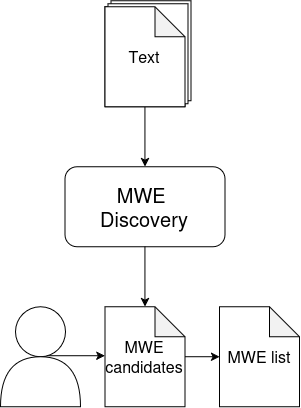
\includegraphics[width=0.8\columnwidth]{../../../FIGURES/phraseology/mwe_discovery.png}
        \end{figure}
    \end{minipage}
\end{frame}

\begin{frame}{MWE Discovery with Association Measure \citep{}} %church and hanks, 1989
    \begin{center}
        \Large
        \begin{equation*}
            I(x, y) = log^2 \frac{P(x,y)}{P(x)P(y)} 
        \end{equation*}
    \end{center}
    \vfill
    \begin{minipage}{0.45\columnwidth}
        \begin{table}
            \centering
            \renewcommand{\arraystretch}{1.5} 
            \begin{tabular}{|p{2cm}|p{2cm}|r|}
                \hline
                computer & scientist & 1.12 \\
                \hline
                keeping  & from      & 2.14 \\
                \hline
                set      & up        & 7.30 \\
                \hline
            \end{tabular}
        \end{table}
    \end{minipage}
    \hfill
    \begin{minipage}{0.45\columnwidth}
        \begin{table}
            \centering
            \renewcommand{\arraystretch}{1.5} 
            \begin{tabular}{|p{2cm}|p{2cm}|r|}
                \hline
                a   & doctor & 0.96  \\
                \hline
                set & about  & -0.60 \\
                \hline
                man & women  & -0.12 \\
                \hline
            \end{tabular}
        \end{table}
    \end{minipage}
\end{frame}

\begin{frame}{MWE Identification}
    \begin{minipage}{0.5\columnwidth}
        \begin{block}{Goals}
            \begin{itemize}
                \item Annotate MWEs in texts
                \item Take variation into account
            \end{itemize}
        \end{block}
        \vfill
        \begin{block}{Methods}
            \begin{itemize}
                \item Rule-based or statistical
                \item Based on a list of expected MWEs
            \end{itemize}
        \end{block}
    \end{minipage}
    \hfill
    \begin{minipage}{0.4\columnwidth}
        \begin{figure}
            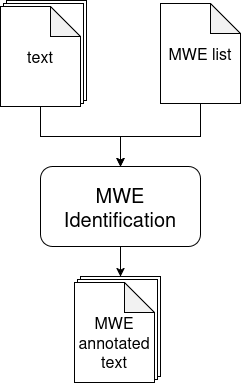
\includegraphics[width=0.7\columnwidth]{../../../FIGURES/phraseology/mwe_identification.png}
        \end{figure}
    \end{minipage}
\end{frame}

\begin{frame}{MWE Identification with Statistical Approaches}
    \begin{figure}
        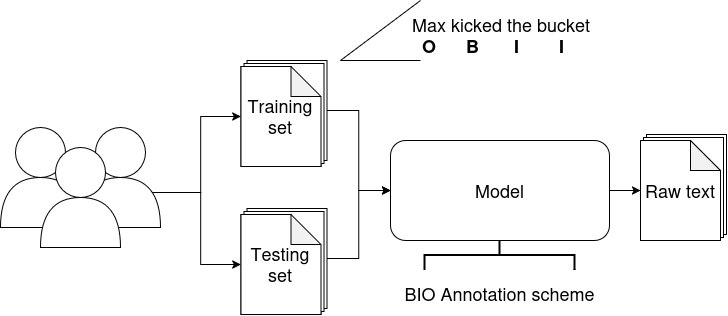
\includegraphics[width=1\columnwidth]{../../../FIGURES/phraseology/statistical_mwe_identification.png}
    \end{figure}
\end{frame}

\begin{exoframe}{Exercise Time !}
    \begin{center}
        \Large
        What about rule-based MWE identification ? \\
        \vspace{10pt}
        Find some rules which might help identificating MWEs in texts.
    \end{center}
\end{exoframe}

\begin{frame}{MWE Identification with Rule-based Approaches}
    \begin{block}{Seen2Seen set of rules \citep{}} % pasquer 2020
        \begin{itemize}
            \item Use lemmas of each word
            \item Use POS tags of each word 
            \item Consider discontinuities (maximum distance between units ?)
            \item Always favor closest components
            \item Units must have syntactic connections
            \item Consider lexical variations
            \item Consider nested MWEs (within each others)
        \end{itemize}
    \end{block}
\end{frame}

\begin{frame}{About Discontinuities}
    \begin{figure}
        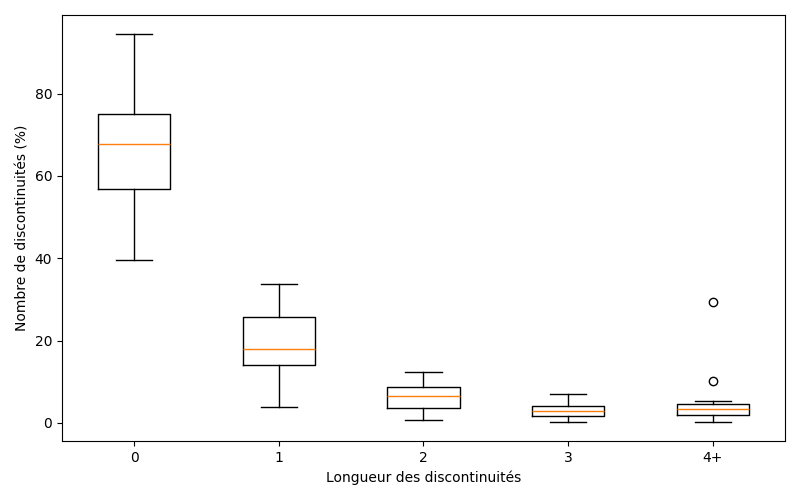
\includegraphics[width=0.7\columnwidth]{../../../FIGURES/phraseology/boxplot_discontinuous_parseme.png}
    \end{figure}
\end{frame}

\begin{frame}{Doggy bag}
    \begin{minipage}{0.45\columnwidth}
        \begin{block}{Multiword Expressions}
            \begin{itemize}
                \item Studied in phraseology
                \item Several components
                \item Somewhat fixed
                \item Somewhat idiomatic
                \item Always conventionalized
            \end{itemize}
        \end{block}
        \begin{block}{MWEs and NLP}
            \begin{itemize}
                \item MWE discovery
                \item MWE identification
            \end{itemize}
        \end{block}
    \end{minipage}
    \hfill
    \begin{minipage}{0.45\columnwidth}
        \begin{figure}
            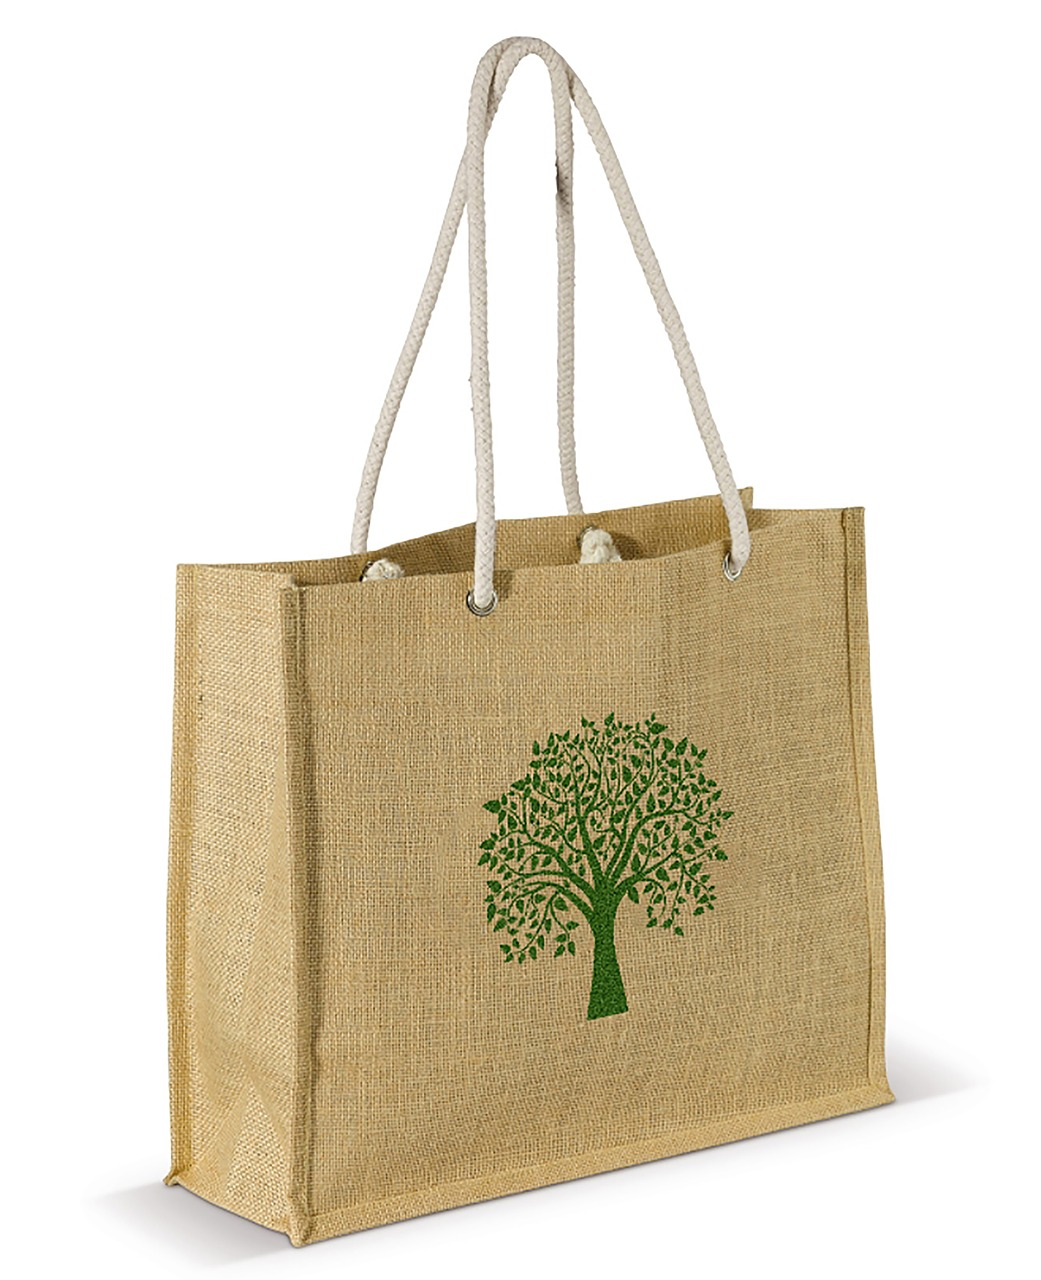
\includegraphics[width=0.9\columnwidth]{../../../FIGURES/divers/doggybag.jpg}
        \end{figure}
    \end{minipage}
\end{frame}

\end{document}



% * : on exam

% > use case: my thesis
% > given a MWE...
% > find its variants

% > why can't I do it with LLMs ?
% > in 2023, they were not as good as today
% > very few works on this matter > no previous work, we should start with basic approaches first => why ?
% > ambitions : making frugal and higly reproductible research

% * focus on the two last points: why starting with basic approaches ? why do i want to make it reproductible => to get the rules, to understand the objects i will be working on, to see the limits of interpretable approaches and question this limit => RESEARCH

% * research is not about finding the most efficient way to solve a task, it is about understanding how things work 

% (Lets say i use a LLM
% it will be better than me at solving the task
% but i wont have a real understanding of why)

% back to my subject: i want to work on defixed MWEs. What should i do ?
% > read the state of the art in both linguistics and NLP => problem: not sota in NLP => find related subjects
% > collect data containing defixed MWEs => where to find such data => social networks, movie names, ...
% > 



% Duh, this class is only interesting for people who want to go in research => this class will give you perspectives that not a lot of engineers and software programmers have
% how can you solve a task if you dont understand it well ? what do you want to do exactly ? the stakes ? 
